%\nonstopmode
\documentclass[%
    a4paper,%
    twoside,%
    BCOR12mm,%
    DIV13,%
    %cleardoubleplain,%
    bibtotoc,%
    openany,%
]{scrartcl}
	\usepackage[ngerman]{babel}
    \usepackage[german]{isodate}
    \usepackage{fontspec}

    \KOMAoptions{draft=on}

    \usepackage{subcaption}

	\usepackage{siunitx}
	\sisetup{
	    locale=DE,
	    separate-uncertainty=true,
        per-mode=symbol,
        range-phrase=%
             \ifmmode\mathbin{-}
             \else%
             { bis }%
             \fi,%
        math-micro=\text{µ},
        text-micro=µ
	}
    \DeclareSIUnit\clight{\ensuremath{c}}

    \usepackage{amsmath}
    \usepackage{unicode-math}

    \usepackage{xfrac}

    \usepackage{booktabs}

    \usepackage{wrapfig}

    \usepackage{hyperref}
    \hypersetup{
        colorlinks,
        citecolor=black,
        filecolor=black,
        linkcolor=black,
        urlcolor=black
    }

    \usepackage{indentfirst}
	% Texteinzug vor Absatz
	\parindent 12pt
    % Schönere Captions
    \usepackage[font=footnotesize,labelfont=bf]{caption}
    \setcapindent{10pt}

    \usepackage[olines]{scrpage2}
    \pagestyle{scrheadings}
    \clearscrheadfoot
    \ofoot[\pagemark]{\pagemark}

    \usepackage[%
        backend=biber,
        sortlocale=de_DE
    ]{biblatex}
    \addbibresource{../00_lit.bib}

    % Einfach \FloatBarrier; Verhindert Bild und Tabellensprünge
    \usepackage[]{placeins}

    \title{%
        V53 -- Mikrowellen auf Hohlleitern
    }
    \author{%
        Kevin Heinicke\\
        \texttt{kevin.heinicke@udo.edu}
        \and
        Markus Stabrin\\
        \texttt{markus.stabrin@udo.edu}
    }

    \date{%
        30. Juni 2014\\
        {\small 1. Abgabe} xx. September 2014
    }
\begin{document}
    \maketitle%
    \tableofcontents
    \newpage
    \section{Theoretische Grundlagen}
\label{sec:theorie}

Dieser Versuch behandelt die Modulation und Demodlation von elektromagnetischen Wellen, um mit Ihnen Informationen von einem Ort
zum anderen übertragen zu können.
Es wird dabei mehr auf die Amplituden- und Frequenzmodulation als Modulationstechnik eingegangen als auf die Phasenmodulation.
Da aus dem modulierten Signal die Informationen wieder rekonstruiert werden müssen, werden auch Demodulationsverfahren angewendet.

\subsection{Amplitudenmodulation}
\label{subsec:klassisch}

Wird die einfachste Form der Amplitudenmodulation betrachtet, so führt die Amplitude einer Hochfrequenten Trägerschwingung $U_\text{T}(t)$ Schwankungen im Rhythmus eines niederfrequenten Modulationssignals $U_\text{M}(t)$ aus.
Mit den dazugehörigen Kreisfrequenzen $\omega_\text{T}$ und $\omega_\text{M}$ und Amplituden $U_\text{0,T}$ und $U_\text{0,M}$ ergibt sich für die Schwingungen
\begin{eqnarray*}
    U_\text{T}(t) &=& U_\text{0,T} \cos{\omega_\text{T} t}\, , \\
    U_\text{M}(t) &=& U_\text{0,M} \cos{\omega_\text{M} t}\, .
\end{eqnarray*}
Damit ergibt sich die amplitudenmodulierte Schwingung 
\begin{equation}
    U_\text{mod}(t) = U_\text{0,T} ( 1 + m \cos{\omega_\text{M} t} ) \cos{\omega_\text{T} t} \label{am:formel1}
\end{equation}
mit dem Modulationsgrad
\begin{equation}
    m = \gamma U_\text{0,M}
\end{equation}
welche einen Wert zwischen 0 und 1 annehmen kann.
Zudem liegt die Amplitude der Schwingung somit zwischen den Extremwerten
\begin{equation}
    U_\text{0,T} (1 \pm m)\,.
\end{equation}
Eine schematische Darstellung der Schwingung ist in Abbildung \ref{am:formel2} dargestellt.

\begin{figure}[!h]
    \centering
    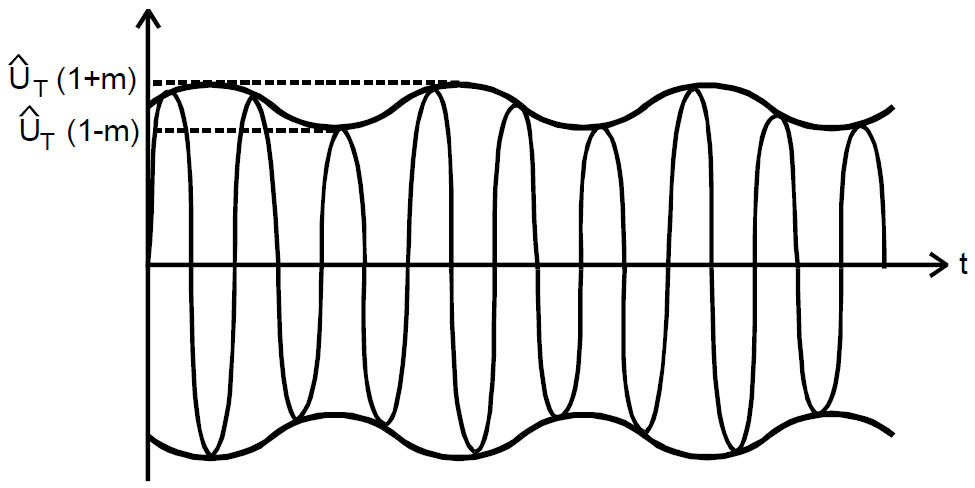
\includegraphics[width=14cm]{images/am-amplitude.png}
    \caption{Zeitabhängigkeit der Momentanspannung $U_\text{mod}(t)$.}
    \label{am:amplitude}
\end{figure}

Mithilfe trigonometrischer Umformulierung ergibt sich aus Gleichung \eqref{am:formel1} 
\begin{equation}
     U_\text{mod}(t) = U_\text{0,T} \left( \cos{\omega_\text{T} t} + \frac{m}{2}\cos{(\omega_\text{T} + \omega_\text{M}) t} + \frac{m}{2}\cos{(\omega_\text{T} - \omega_\text{M}) t}\right) \,. \label{am:formel2}
\end{equation}

Daraus ist zu erkennen, dass das Frequenzspektrum einer in dieser Art und Weise modelierten Schwingung aus 3 Linien mit den Kreisfrequenzen $\omega_\text{T} + \omega_\text{M}$, $\omega_\text{T} - \omega_\text{M}$ und $\omega_\text{T}$ besteht.
$\omega_\text{T}$ überträgt dabei keinerlei Informationen, da sie nicht von der Modulationsamplitude $U_\text{0,M}$ abhängt.
In der Praxis wird daher versucht diese zu unterdrücken, da diese mit einem unnötigen Energieverbrauch verbunden ist.
Da die gesamte Information bereits in einem Seitenband steckt - bei mehreren Frequenzen in der Modulationsspannung verbreitern sich die äußeren Linien zu Frequenzbändern - kann mithilfe eines geeigneten Bandpassfilters bereits im Modulationsprozess eine Seite unterdrückt werden.

Nachteile der Amplitudenmodulation sind die geringe Störsicherheit und die geringe Verzerrungsfreiheit.

\subsection{Frequenzmodulation}
\label{subsec:einstein}

Eine frequenzmodulierte Schwingung kann durch Gleichung
\begin{equation*}
    U(t) = U_\text{0} \sin{\left( \omega_\text{T} t + m \frac{\omega_\text{T}}{\omega_\text{M}} \cos{\omega_\text{M} t} \right)}
\end{equation*}
dargestellt werden.
Die Momentanfrequenz $f$ ergibt sich durch Ableiten des Arguments der Sinusfunktion zu
\begin{equation*}
    f(t) = \frac{\omega_\text{T}}{2 \pi} ( 1 - m \sin{\omega_\text{M} t}) \,.
\end{equation*}
Der Vorfaktor der Sinusfunktion $\frac{m \omega_\text{T}}{2 \pi}$ wird als Frequenzhub bezeichnet und gibt die Variationsbreite der Schwingungsfrequenz an.
Im folgenden soll nur der Fall der Schmalband-Frequenzmodulation (niedriger Frequenzhub) betrachtet werden, also 
\begin{equation*}
    m \frac{\omega_\text{T}}{\omega_\text{M}} \ll 1\,.
\end{equation*}
Ein Beispiel für eine frequenzmodulierte Schwingung ist in Abbildung \ref{fm:modulation} dargestellt.

\begin{figure}[!h]
    \centering
    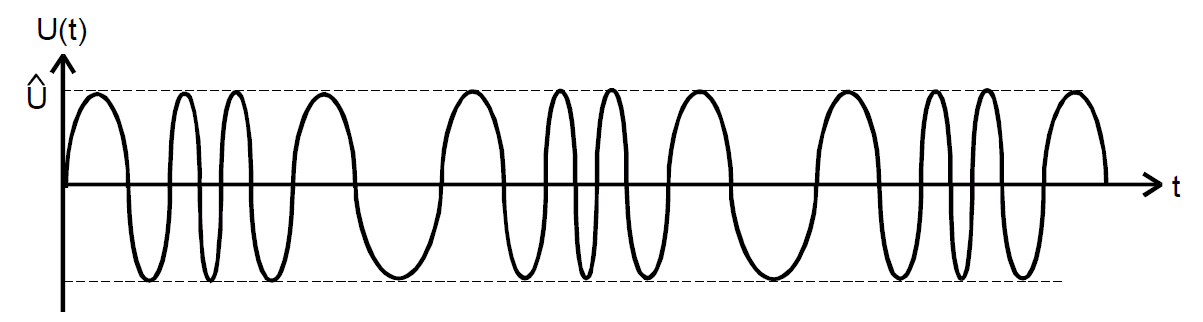
\includegraphics[width = 14cm]{images/fm-modulation.png}
    \caption{Zeitlicher Verlauf einer sinusförmig frequenzmodulierten Schwingung}
    \label{fm:modulation}
\end{figure}

Auch hier ist das Frequenzspektrum recht einfach was an der umgeformten Gleichung 
\begin{equation*}
    U(t) = U_\text{0} \left( \sin{\omega_\text{T} t}\cos{\left(m\frac{\omega_\text{T}}{\omega_\text{M}} \cos{\omega_\text{M} t}\right)} + \cos{\omega_\text{T} t}\sin{\left(m\frac{\omega_\text{T}}{\omega_\text{M}} \cos{\omega_\text{M} t}\right)} \right)\,.
\end{equation*}

Für eine schwach frequenzmodulierte Schwingung ergibt sich somit näherungsweise
\begin{equation*}
    U(t) \approx U_\text{0} \left( \sin{\omega_\text{T} t} + \frac{m \omega_\text{T}}{2 \omega_\text{M}} \cos{(\omega_\text{T} + \omega_\text{M}) t} + \frac{m \omega_\text{T}}{2 \omega_\text{M}} \cos{(\omega_\text{T} - \omega_\text{M}) t}\right) \,,
\end{equation*}
woraus sich wieder drei Teilschwingungen wie bei der amplitudenmodulierten Schwingung ergeben.
Der Unterschied liegt darin, dass die Trägerschwingung gegen die beiden Seitenlinien um $\frac{\pi}{2}$ verschoben ist.

\subsection{Modulationsschaltungen}
\label{subsec:debye}

\subsection{Demodulator - Schaltungen}
\label{subsec:debye}

\section{Durchführung}
\label{sec:durchführung}

    \section{Messung} % (fold)
\label{sec:messung}
Im Folgenden Abschnitt werden die Messungen der Gitterkonstante von HOPG, sowie
der Plateauhöhen von Gold erläutert. Zum einlesen der Messdaten und für eine
einfache Rauschunterdrückung wird die freie Software \texttt{gwyddion}
\cite{gwyddion} benutzt. Für die Analyse wird \texttt{python} \cite{python3}
verwendet.

Um mit dem Mikroskop verwertbare Bilder zu erzeugen, muss zunächst eine Stück
Wolframdraht mit einer Zange abgetrennt werden. Dabei ist es essentiell, den
Draht abzureissen, statt ihn abzuschneiden. Dadurch wird gewährleistet, dass
ein Ende des Drates eine sehr feine -- im Idealfall einatomige -- Spitze
aufweist.

Die Spitze wird in den Mikroskopschlitten eingelegt und die Probe mit Hilfe von
Piezzoelementen an diese herangefahren. Die Steuerung wird mit Hilfe der dem
Mikroskop beiliegenden Software \emph{Zitation einfügen} durchgeführt.
Sobald der Abstand so klein ist, dass ein Tunnelstrom gemessen wird, fährt
die Probe ein zuvor definiertes Raster in $x$- und $y$-Richtung ab. Das so
entstehende Bild wird gespeichert und ausgewertet.

\subsection{Gittervektoren von HOPG}
\label{subsec:gitter}
Zunächst werden einige Testaufnahmen erstellt, um Mikroskopeinstellungen zu
finden, die die zu untersuchende Gitterstruktur erkennen lassen.
Der Bildausschnitt deckt dabei eine Fläche von $\num{2}\times\num{2}\,
\si{\nano\meter\squared}$ ab. Die Aufnahme, nach Vorverarbeitung durch
\texttt{gwyddion}, ist in Abbildung \ref{fig:hopg1} dargestellt.
\begin{figure}
    \centering
    \includegraphics[width=0.5\linewidth]{build/plots/HOPG_downwards.pdf}
    \caption{Aufnahme von Graphit mit dem Rastertunnelmikroskop. Eine
             periodische Struktur ist klar zu erkennen.}
    \label{fig:hopg1}
\end{figure}
Offensichtlich taucht bei $x \approx \SI{1.05}{\nano\meter}$ eine Unstetigkeit
auf. Außerdem ist die Aufnahme im Bereich $y > \SI{1.5}{\nano\meter}$
anscheinend verzerrt. Diese Werte werden als grobe Selektion der Daten
benutzt, mit denen die Gittervektoren bestimmt werden.

In einem nächsten Schritt werden alle lokalen Maxima in einer Umgebung von
\num{12} Pixeln gesucht und markiert. Im zuvor gewählten Selektionsbereich
werden zudem zwei Korridore mit möglichst vielen Maxima gewählt, die sich an
der grob zu erkennenden Struktur der Gitterstruktur orientieren.
Die grobe Vorselektion, die Maxima und die Selektionskorridore sind in
Abbildung \ref{fig:hopg1_selektion} dargestellt.
An die Punkte innerhalb dieser Korridore werden in einem Least-Squares-Fit
lineare Funktionen angepasst und damit Richtungsvektoren bestimmt. Die Länge
dieser Vektoren wird duch Mittelung über alle benutzten Punkte bestimmt.
Dabei werden zwei Gittervektoren $\vec{a}_1$ und $\vec{a}_2$ der Hexagonalen
Struktur, sowie ein Vektor des Ebenenabstandes $\vec{b}$ bestimmt.
Die Vektoren sind in Abbildunge \ref{fig:hopg1_vektoren} eingezeichnet und
haben die Werte
\begin{align*}
    \input{build/tex/down_vec_a.tex} \qquad &\text{mit} \qquad
    \input{build/tex/down_vec_a_len.tex}\,,\\
    \text{und}\qquad\input{build/tex/down_vec_b.tex} \qquad &\text{mit}\qquad
    \input{build/tex/down_vec_b_len.tex}\,.
\end{align*}
Der Winkel zwischen den Vektoren beträgt
\begin{align*}
    \input{build/tex/down_angle.tex}\,.
\end{align*}
Durch Vergleich mit den Literaturwerten \cite{HOPG_gittervektoren} $\hat{a}
= \SI{2.461}{\angstrom}$ und dem erwarteten Winkel $\alpha = \SI{60}{\degree}$
lässt sich
eine Skalierung der $x$- und $y$- Achse finden, sodass die gemessenen Werte
für $\left|\vec{a}_i\right|$ mit diesen
übereinstimmen.
\begin{figure}
    \centering
    \subcaptionbox{
        Grobe Vorselektion der zum Fitten genutzten Datenpunkte.
        \label{fig:hopg1_selektion}
    }[0.6\linewidth]{\includegraphics[width=0.57\linewidth]{build/plots/hopg_down_selection.pdf}}
    \subcaptionbox{
        Gefittete Gittervektoren.
        \label{fig:hopg1_vektoren}
    }[0.39\linewidth]{\includegraphics[width=0.42\linewidth]{build/plots/hopg_down_arrows.pdf}}
    \caption{Vorselektion und Fitresultate der Bestimmung der Gittervektoren.}
    \label{fig:hopg_fit}
\end{figure}

\subsection{Plateauhöhen einer Goldoberfläche}
\label{subsec:gold}

\clearpage
\section{Diskussion}
\label{sec:diskussion}

    \printbibliography
\end{document}
